\documentclass[12pt]{article}

\usepackage{amssymb,amsmath,amsfonts,eurosym,geometry,ulem,graphicx,caption,color,setspace,sectsty,comment,footmisc,caption,natbib,pdflscape,subfigure,array,hyperref}
\usepackage{indentfirst}

\normalem

\onehalfspacing
\newtheorem{theorem}{Theorem}
\newtheorem{corollary}[theorem]{Corollary}
\newtheorem{proposition}{Proposition}
\newenvironment{proof}[1][Proof]{\noindent\textbf{#1.} }{\ \rule{0.5em}{0.5em}}

\newtheorem{hyp}{Hypothesis}
\newtheorem{subhyp}{Hypothesis}[hyp]
\renewcommand{\thesubhyp}{\thehyp\alph{subhyp}}

\newcommand{\red}[1]{{\color{red} #1}}
\newcommand{\blue}[1]{{\color{blue} #1}}

\newcolumntype{L}[1]{>{\raggedright\let\newline\\arraybackslash\hspace{0pt}}m{#1}}
\newcolumntype{C}[1]{>{\centering\let\newline\\arraybackslash\hspace{0pt}}m{#1}}
\newcolumntype{R}[1]{>{\raggedleft\let\newline\\arraybackslash\hspace{0pt}}m{#1}}

\geometry{left=1.0in,right=1.0in,top=1.0in,bottom=1.0in}

\begin{document}

\begin{titlepage}
\title{Predictions on TARGET2 Balance}
\author{Sherry Peng Tian\thanks{Tian: Boston College, tianpe@bc.edu, Eagle ID: 1675 1338}}
% \and Surname2\thanks{affiliation2, address2, email2. Acknowledgements}}
\date{\today}
\maketitle
\begin{abstract}
\noindent Placeholder\\
\vspace{0in}\\
\noindent\textbf{Keywords:} seasonal naïve methods, simple forecasting, TARGET2 balance\\
\bigskip
\end{abstract}
\setcounter{page}{0}
\thispagestyle{empty}
\end{titlepage}

\pagebreak \newpage

\doublespacing

%\clearpage
%\section*{Figures} \label{sec:fig}
%\addcontentsline{toc}{section}{Figures}

%\begin{figure}[hp]
%  \centering
%  \includegraphics[width=.6\textwidth]{../fig/placeholder.pdf}
%  \caption{Placeholder}
%  \label{fig:placeholder}
%\end{figure}
%\clearpage


\section{Background} \label{sec:background}

European Union, as the largest monetary organization and the second largest economy in nominal terms (only after the United States) according to GDP, PPP, and nominal GDP, those normally accepted economic measures, was established in November, 1993. EU countries gather together to make determination on economic policies, environmental issues, political pointviews, and even educational and employment development. Therefore, the study of the EU economy assists in the long run of understanding and predicting the global trend of economic development. Starting from the year of 1999 with some EU member states, now 19 out of 28 EU states/countries accept and use euro as official and main currency in a currency union (called Eurozone); however the remaining 9 states still accept the usage of euro in some ways, making euro the most widely used currency in the EU. 

TARGET2 stands for Trans-European Automated Real-time Gross settlement Express Transfer system and works as a settlement system for the Eurozone. It is based on an integrated central technical infrastructure, called the Single Shared Platform (SSP), which is operated by three central banks of France, Germany, and Italy. Beginning in November 2007, TARGET2 starts to replace TARGET and is made accessible to members outside of the Eurozone countries. Since TARGET2 works as an interbank real-time gross settlement payment system for the clearing of cross-border transfers in the Eurozone, the objectives includes supporting EU monetary policy, stablizing Eurozone money market, minimizing systemic risk and increasing the efficiency of cross-border transfers. Understanding and accurately predicting of TARGET2 balance can establish a good foundation about the global economics. 

Since the Eurozone monetary system consists of the European Central Bank (ECB) and the national central banks of all 19 EU member states, a well-balanced TARGET2 system should be the national commercial banks supporting investment and consumption while maintaining a clear transaction with the national central bank, and then the central banks of different countries linking to ECB via TARGET system, left with parties of creditor nations and borrower nations. When a Eurozone country has a balanced national payment, its TARGET2 balance equals to zero, but when a country encounters unwilingness of equity financing or the expectation of macroeconomics is inclined to drop, the country lacks the capability to pay debts back and becomes the debitor nation, resulting in the creditor nation with a positive TARGET2 balance. During the financial crisis, the After the 2008 financial crisis, the Eurozone monetary market recovers from the higher pressure of subprime financial debts around 2012. 

\section{Literature Review} \label{sec:literature}
\subsection{Interpreting TARGET2 balances}
Even though TARGET2 balance usually is seen as a safety net indicator between the ECB and national central banks, the rise in TARGET2 of German Bundesbank brings deeper concern of more appropriate interpretation and policy response. The article proposes two different ideas of the TARGET2 balances as "flow interpretation" corresponding to the current account financing and as "stock interpretation" of financing the reversal of an outstanding stock of cross-border to solve a balance of payments crisis. To sum up the arguments, the changes in TARGET2 balances come financing current account deficits, shifting stocks of financing, and hedging redonomination risks. Meanwhile, the interpretation of T-balance could be hugely different before or after the financial crisis, because from the balance sheets and identities, the pre-crisis mechanism depends mainly on the ECB's full allotment refinancing operations to maintain the balance of payments identity: 
\begin{equation*}
\text{Current account} + \text{Capital account} + \text{Official settlements balance} = 0 
\end{equation*}
Therefore, if there is a gold standard or other fixed exchange rate regime like Hong Kong SAR exists, TARGET2 balance, resulting from the changes in foreign exchange reserves, will show up. Moreover, financial risks, financing deficits, and many other reasons from financial crisis stress put reversal forces on TARGET2 to be more positive. At the end, the journal article evaluates three policy issues raised by that discussion: appropriate balance between financing and adjustment of current accounts, risks taken on by private credit exposur (or the credit reversal reversed), and discouraging positioning against euro by private parties. 

\subsection{What are the drivers of the large TARGET2 balances}
This paper examimes the extent to which changes in national TARGET2 balances can be statiscally associated wiht cross-border private capital flows and current account (CA) balances around the financial crisis in 2007. The data used for statistically analysis is a panel quarerly dataset from 1999 to 2012 in 12 Eurozone countries. It is shown that current balance and changes in T2 balances were not related until the start of the 2007 financial crisis, and the relation has become statistically significant and economically sizeable after then. As related literature meantioned how sudden stop like financial crisis shock and private capital flows will influence the trend distribution, one of the conclusions is that there is no evidence that the institutional set-up of the ECB is fundamentally flawed or will ever lead to ever-increasing imbalances. The second conclusion is that TARGET2 balances should not be settled or limited, but instead, the focus should be harmonizing long-term collateral policies. 

\subsection{Measuring Economic Policy Uncertainty}
This journal introduces a new index of economic policy uncertainty (EPU) covering major financial events after late 1930s. The approach to establishing indices is based on human-reading newspaper coverage frequency and then captures the policy principals, methods, and outcomes. Meanwhile, the indices include categories such as, the Fed, central banks, interest rate, inflation, and etc, based on differentiation of vocabulary. As for human-readings, the paper evaluates the process at the end with an audit study: the researchers spent six months developing an audit process designed for US EPU indices and another 18 months running a large-scale human audit study to ensure correctness. Additionally, the pilot audit was done with student research assistants, who read and coded randomly selected newspaper articles. 

\subsection{Does the Box–Cox transformation help in forecasting macroeconomic time series? }
As the title indicates, this paper evaluates whether transforming a time series leads to an improvement in forecasting accuracy. The Box-Cox power transformation is widely used in econometrics and measured on a ratio scale. The experimental datasets include a large set of seasonal monthly macroeconomic time series related to industrial prodcution and retail turnover and a nonparametric experiement for estimating the optimal transformation parameters. Box and Cox (1964) proposed a transformation of a time series variable $y_t, t = 1, ..., n$ that depends on the power parameter $\lambda$ in the following way: 
$$
y_t(\lambda) = 
  \begin{cases}
    \frac{y_t^{\lambda} - 1}{\lambda}, &\quad \lambda \neq 0, \\ 
    \ln{y_t}, &\quad \lambda = 0. 
  \end{cases}
$$
The naïve forecast is obtained as the inverse Box-Cox tranformation, 
$$
\hat{y_{t+h|t}} = 
  \begin{cases}
    (1+\lambda \tilde{y}_{t+h|t}(\lambda)^{1/\lambda}), &\quad \lambda \neq 0, \\
    \exp(\tilde{y}_{t+h|t}(\lambda)), &\quad \lambda = 0. 
  \end{cases} 
$$
corresponding to the median of the predictive distribution; hence, it provides the minimum absolute error predictor, when the condition that the transformed series has to be normally distributed is needed. After a sequences of mathmatical deduction and empirical experiments, it reaches three conclusions: first is that the Box-Cox transformation can explain roughly one fifth of the series, so the implementation of Box-Cox and even log transformation can improve the forecast accuracy; the second is that the forecast comparison shows that transformations can improve the forecast accuracy rate at short horizons, but the advantage of using diminishes for the longer-term; the third is that their nonparametric approach frankly provide good guidance when researcher don't or cannot satisfy three assumptions of Box-Cox transformation. 

\subsection{A comparison of forecasting methods for hotel room occupancy}
The significance of this journal article is that simple methods like naïve forecasting and seasonal naïve method are investigated and evaluated as well as the accuracy evaluation measures we learned in class. Even though there are a few types of forecasting categories that have been used such as hotel room occupancy forecast, implementation of this forecasting category can be crucial because it leads to an efficient planning for, and decision making to all the hotel departments. Thus, the study aims to compare the best forecasting method for hotel room occupancy. Therefore, Seasonal Naïve, Seasonal Holt Winter’s Method and ARIMA are implemented in order to determine which forecasting method is most suitable to forecast hotel room occupancy by using secondary data from year 2012 until 2017. The selection of best method is based on three error measurements which are root mean square error (RMSE), mean absolute percentage error (MAPE) and mean absolute error (MAE). From the analysis conducted, the results show the best method to be implemented is the Seasonal Holt Winter’s Multiplicative method since it shows the lowest error for all three measurements. Furthermore, the forecast of future hotel room occupancy for year 2018 shows similar pattern as previous years. In comparing 2018 future occupancy with 2017 actual occupancy, there are some increment and decrement in hotel room occupancy for various months.

\subsection{Time Series Seasonal Adjustment Using Regularized Singular Value Decomposition}

\section{Model} \label{sec:model}
\subsection{Data Source and Cleaning}
The policy uncertainty index of various countries is derived directly from \href{https://www.policyuncertainty.com/monetary.html}{\underline{Economic Policy Uncertainty}} website and the TARGET2 balance datasets are from \href{http://www.eurocrisismonitor.com}{\underline{Institute of Empirical Economic Research}} at Osnabrück University, which is a reliable source for tracking TARGET2 balances from Janurary 1987 to June 2019, updated nearly on a monthly basis. 

Since the timelines of two datasets are moduled the same, after year and month, there is no difficulty transferring the combined ones into a time series. Refererring to the raw dataset, there are missing variables only for ECB and Cyprus groups. Table 1 below has shown descriptive details of countries' TARGET2 balance as well as the policy uncertainly index from a macroeconomic perspective. In addition, Figure 1 of uncertainly index has shown that most index lie below 200 with some extreme values extending to 1000. The policy uncertainty is measured using political news and macroeconomic events in 100 percentage. The extreme higher index of United Kingdom and France can be explained by the event of Brexit and the discussion around exiting from the EU. Figure 2 shows the median ranking of TARGET2 Balance, which corresponds to people's usual understanding. Figure 3 displays the only two negative examples of Austria and Begium, where the balance from 2001 till now has been below zero. The significance of this paper, one is to help understand the main components of policy uncertainty indices and various weights on financial incidents; the other is to create new measures for 12 different economies, including US and UK. 
\begin{table}[!htbp] \centering 
  \caption{Descriptive statistics} 
  \label{} 
  \resizebox{1\textwidth}{!}{
\begin{tabular}{@{\extracolsep{5pt}} ccccc} 
\\[-1.8ex]\hline 
\hline \\[-1.8ex] 
 & mean & sd & min & max \\ 
\hline \\[-1.8ex] 
Austria & -24296.7933783784 & 14674.3237811389 & -46049.49 & 4086.61 \\ 
Belgium & -23289.5541891892 & 19329.5564321393 & -98312.13 & 7687.79 \\ 
Cyprus &  &  &  &  \\ 
ECB &  &  &  &  \\ 
European-News-Index & 154.548700315458 & 66.3208691016548 & 47.6923446655273 & 433.277496337891 \\ 
France & 185.035862158011 & 98.0282374243346 & 30.6203689575195 & 574.633178710938 \\ 
France-News-Index & 185.035862158011 & 98.0282374243346 & 30.6203689575195 & 574.633178710938 \\ 
Germany & 137.807954985816 & 65.0741829256057 & 28.4339847564697 & 454.005432128906 \\ 
Germany-News-Index & 137.807954985816 & 65.0741829256057 & 28.4339847564697 & 454.005432128906 \\ 
Greece & 102.636670389217 & 26.6825469949835 & 47.1814761087496 & 188.704530504278 \\ 
Greece-policy-uncertainty & 123.493935990991 & 60.0910694754914 & 28.63219 & 344.2343 \\ 
Ireland & 121.966938633335 & 55.9441890855816 & 22.9658655600782 & 282.127765252969 \\ 
Italy & 110.990210017642 & 38.5988775008311 & 31.7015342712402 & 241.018203735352 \\ 
Italy-News-Index & 110.990210017642 & 38.5988775008311 & 31.7015342712402 & 241.018203735352 \\ 
Netherlands & 95.8721697437445 & 38.2458191255031 & 27.2133611447053 & 233.73110601772 \\ 
Spain & 109.835684836893 & 32.7956285430677 & 56.2692222595215 & 236.578872680664 \\ 
Spain-News-Index & 112.530257319545 & 57.697184778201 & 23.3175201416016 & 407.419403076172 \\ 
Sweden & 91.4955742387561 & 18.6321694506138 & 53.73406929 & 156.7298215 \\ 
UK & 209.477777781787 & 156.802512055422 & 30.4688014984131 & 1141.79553222656 \\ 
UK-News-Index & 209.477777781787 & 156.802512055422 & 30.4688014984131 & 1141.79553222656 \\ 
\hline \\[-1.8ex] 
\end{tabular}} 
\end{table} 
\begin{figure}
  \centering 
  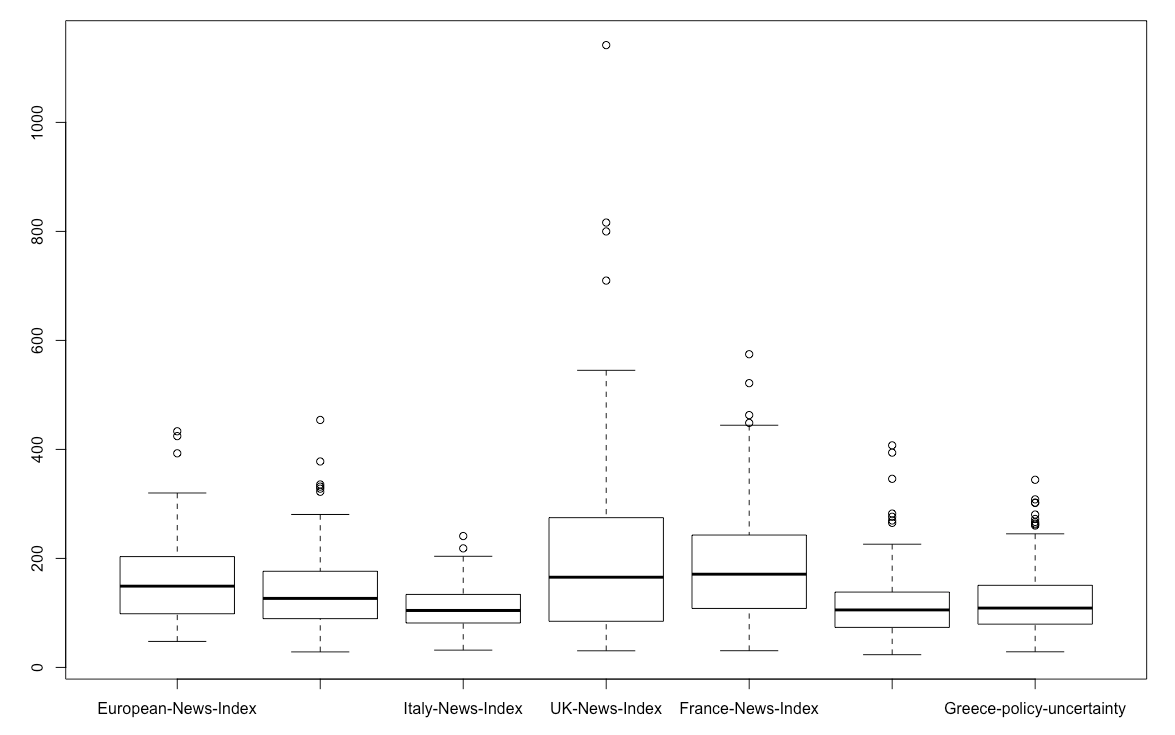
\includegraphics[width=\linewidth]{Uncertainty.png}
  \caption{European, Germany, Italy, UK, France, Spain, Greece News Index}
  \label{fig:policy_uncertainty}
\end{figure}

\begin{figure}[!tbp]
  \centering
  \begin{minipage}[b]{0.5\textwidth}
    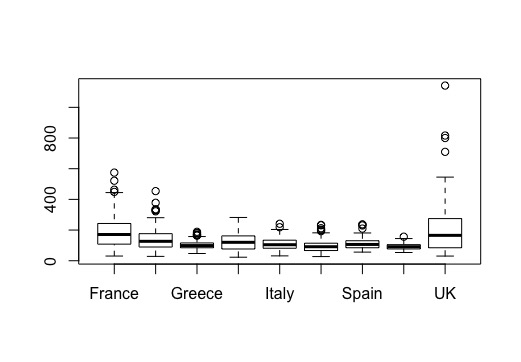
\includegraphics[width=\textwidth]{Bal1.jpeg}
    \caption{Target2 of France, Germany, Greece, Ireland, Italy, Netherlands, Spain, and UK}
  \end{minipage}
  \hfill
  \begin{minipage}[b]{0.4\textwidth}
    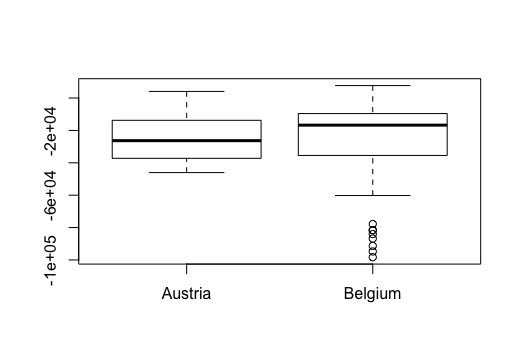
\includegraphics[width=\textwidth]{Bal2.jpeg}
    \caption{Negative Target2 Balance of Austria and Belgium}
  \end{minipage}
\end{figure}
For the purpose of prediction on TARGET2 Balance, the time intervals are parsed from the year 2001 because the transition of millennial, even though the financial crisis around 2008 has also seriously influenced the economics and our further prediction. Furthermore, for any need of calculating the accuracy, the test datasest is splitted from Janurary 2015 to June 2019. As Figure 4 indicates the train-test split visually. 
\begin{figure}
  \center
  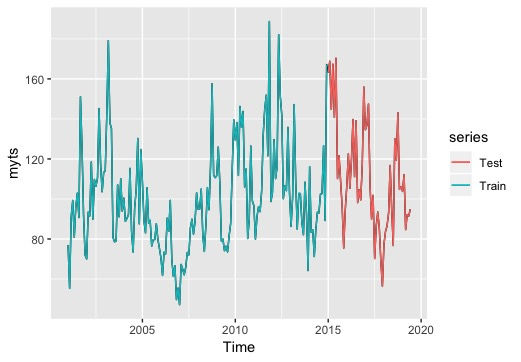
\includegraphics[width=0.8\linewidth]{split.jpeg}
  \caption{Greece TARGET2 Train Test Split}
  \label{fig:split}
\end{figure}

\subsection{Transformation and Decomposition}
Understanding the systematic overall patterns is important, given that the literature on TARGET2 imbalances raise high attention to the timeline of financial crisis. There has not been an established view of point regarding causual relationships of T2; therefore, the study could be deviated from the strucuture of the entire European Monetary System to a single particular country, which Greece is picked under these circumstances. Firstly, the additive decomposition of Greece balance from 2001 to June 2019 shows that there might not be a clear trend but there is a clear seasonality occuring every year. Moreover, the multiplicative decomposition shows the same just with a smoother trend line (Figure 5 and Figure 6). 
\begin{figure}[!tbp]
  \centering
  \begin{minipage}[b]{0.49\textwidth}
    \includegraphics[width=\textwidth]{Additive.png}
    \caption{Additive Decomposition of Greece TARGET2 Balance}
  \end{minipage}
  \hfill
  \begin{minipage}[b]{0.49\textwidth}
    \includegraphics[width=\textwidth]{Multiplicative.png}
    \caption{Multiplicative Decomposition of Greece TARGET2 Balance}
  \end{minipage}
\end{figure}

Data transformation is needed to create a smooth line or a normal distribution to further help with the forecasting methods. The Box-Cox transformation gives a normal distribution and smoother trend to the initial distribution. Using the systematic calculated lambda of -0.416, it improves the distribution shape after transformation, which we could use for ARIMA model later. 

\subsection{Seasonal Naïve Method}
\begin{figure}[!tbp]
  \centering
  \begin{minipage}[b]{0.49\textwidth}
    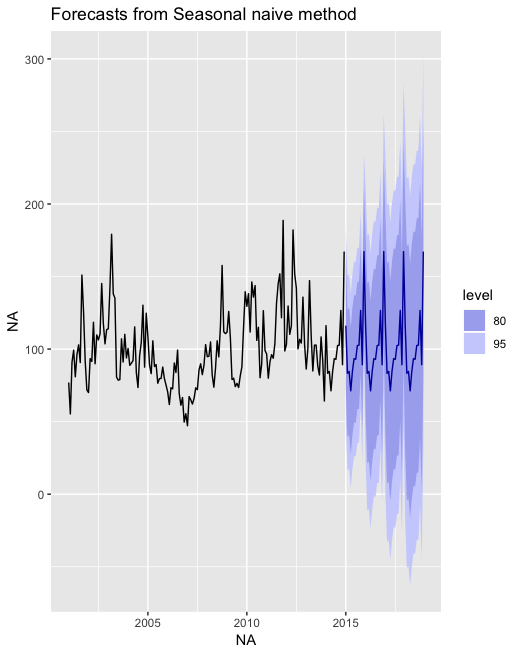
\includegraphics[width=\textwidth]{Pre_sn.png}
    \caption{Seasonal Naïve Forecast}
  \end{minipage}
  \hfill
  \begin{minipage}[b]{0.49\textwidth}
    \includegraphics[width=\textwidth]{residuals.png}
    \caption{Residuals Check for Seasonal Naïve Method}
  \end{minipage}
\end{figure}
After trying several simple methods we have learned in class so far, since there is a clear seasonal trend from the previous decomposition, the most accurate forecast method is seasonal naïve. According to Figure 8, the residuals are normally distributed and deviating around zero, even though there is loads of white noise, showing in the autocorrelation graph. Figure 7 shows the forecast outcome based on train sets with confidence intervals of 80 and 95 percentage. The accuracy result is following in Table 2: 
\begin{table}[!htbp] \centering 
  \caption{} 
  \label{} 
\begin{tabular}{@{\extracolsep{5pt}} ccccccccc} 
\\[-1.8ex]\hline 
\hline \\[-1.8ex] 
 & ME & RMSE & MAE & MPE & MAPE & MASE & ACF1 & Theil's U \\ 
\hline \\[-1.8ex] 
Training set & $0.519$ & $34.211$ & $26.837$ & $$-$4.655$ & $26.768$ & $1$ & $0.533$ & $$ \\ 
Test set & $11.127$ & $41.438$ & $32.193$ & $2.670$ & $29.269$ & $1.200$ & $0.547$ & $1.939$ \\ 
\hline \\[-1.8ex] 
\end{tabular} 
\end{table} 

\section{Next Things}

With more understanding of other uncertainty index and other factors, there could include some regressors and apply time-series multi-regression to the model. Additionally, data transformation and more complex forecasting methos are needed and will be learned to improve the forecast accuracy. 
%\section{Results} \label{sec:result}

%\section{Conclusion} \label{sec:conclusion}

%\section*{Tables} \label{sec:tab}
%\addcontentsline{toc}{section}{Tables}
\singlespacing
\setlength\bibsep{0pt}
\bibliographystyle{my-style}
\bibliography{APA}

\clearpage

\onehalfspacing

\section*{Appendix: References} \label{sec:references}
\addcontentsline{toc}{section}{Appendix: References}

Baker, Scott, Bloom, Nicholas and Davis, Steven, (2016), Measuring Economic Policy Uncertainty, The Quarterly Journal of Economics, 131, issue 4, p. 1593-1636, https://EconPapers.repec.org/RePEc:oup:qjecon:v:131:y:2016:i:4:p:1593-1636..

Cecchetti, Stephen G. and McCauley, Robert N. and McGuire, Patrick M., Interpreting TARGET2 Balances (December 1, 2012). BIS Working Paper No. 393. Available at SSRN: https://ssrn.com/abstract=2195965 

Desa, N., and Marzuki. (2019). A comparison of forecasting methods for hotel room occupancy. AIP Conference Proceedings, 2138(1), The 4th Innovation And Analytics Conference and Exhibition (Iace 2019), Kedah, Malaysia (25–28 March 2019):.

Juan, Barredo-Zuriarrain and Ricardo Molero-Simarro and Alejandro Quesada-Solana, 2017. "Euro-dependence — a peripheral look beyond the Monetary union : a proposal of reform of the TARGET2," Post-Print halshs-01585803, HAL. <https://ideas.repec.org/p/hal/journl/halshs-01585803.html>. 

Raphael A. Auer, 2013. "What Drives TARGET2 Balances? Evidence from a Panel Analysis," CESifo Working Paper Series 4216, CESifo Group Munich. <https://ideas.repec.org/p/ces/ceswps/\_4216.html>. 

Wei Lin, Jianhua Z. Huang and Tucker McElroy (2019) Time Series Seasonal Adjustment Using Regularized Singular Value Decomposition, Journal of Business and Economic Statistics, DOI: 10.1080/07350015.2018.1515081

Proietti, Tommaso and Lütkepohl, Helmut, 2006. Does the Box-Cox transformation help in forecasting macroeconomic time series? Merewether Building (H04), Discipline of Business Analytics, The University of Sydney. NSW 2006, Australia. International Journal of Forecasting 29 (2013) 88-99. 

\end{document}